\section{Référence de la classe IterateurBidir}
\label{class_iterateur_bidir}\index{IterateurBidir@{IterateurBidir}}
Graphe d'héritage de IterateurBidir::\begin{figure}[H]
\begin{center}
\leavevmode
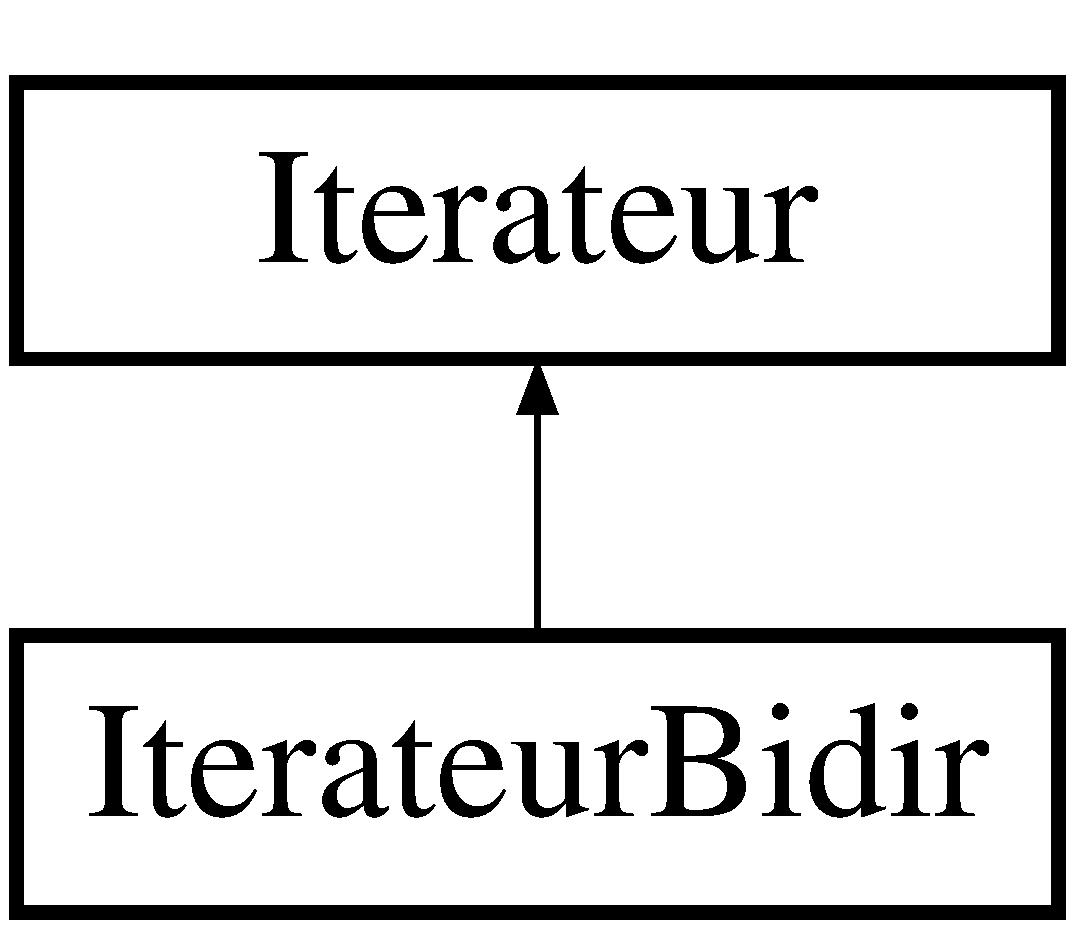
\includegraphics[height=2cm]{class_iterateur_bidir}
\end{center}
\end{figure}


\subsection{Description détaillée}
Interface exigeant une méthode supplémentaire par rapport aux itérateurs \char`\"{}simples\char`\"{}, afin d'implémenter des itérateurs bidirectionnels. \subsection*{Fonctions membres publiques}
\begin{CompactItemize}
\item 
{\bf prec} ()\label{class_iterateur_bidir_c168276a3bf249dc56d2287e7c07455e}

\begin{CompactList}\small\item\em Déplace l'itérateur d'une position vers l'arrière. \item\end{CompactList}\end{CompactItemize}


La documentation de cette classe a été générée à partir du fichier suivant :\begin{CompactItemize}
\item 
src/lib/std/{\bf IterateurBidir.php}\end{CompactItemize}
